\documentclass[11pt,a4paper]{report}
\usepackage[all]{nowidow}
\usepackage{preamble}
\usepackage[T1]{fontenc}
\usepackage{titlesec, blindtext, color}
\definecolor{gray75}{gray}{0.75}
\newcommand{\hsp}{\hspace{20pt}}
\titleformat{\chapter}[hang]{\Huge\bfseries}{\thechapter\hsp\textcolor{gray75}{|}\hsp}{0pt}{\Huge\bfseries}
\usepackage{xcolor}
\usepackage{listings}
\usepackage{enumitem}
\usepackage{minted}
\usepackage{pdfpages}
\usepackage{pdflscape}
\usepackage{titlesec}
\usepackage{changepage}

\titlespacing*{\section}{0pt}{0.5\baselineskip}{0.5\baselineskip}
\titlespacing*{\chapter}{0pt}{0.7\baselineskip}{0.7\baselineskip}

\graphicspath{ {figures/} }
\newcommand\note[1]{\textcolor{red}{#1}}
\newcommand\JSONnumbervaluestyle{\color{blue}}
\newcommand\JSONstringvaluestyle{\color{red}}
% switch used as state variable
\newif\ifcolonfoundonthisline

\makeatletter

\lstdefinestyle{json}
{
  showstringspaces    = false,
  keywords            = {false,true},
  alsoletter          = 0123456789.,
  morestring          = [s]{"}{"},
  stringstyle         = \ifcolonfoundonthisline\JSONstringvaluestyle\fi,
  MoreSelectCharTable =%
    \lst@DefSaveDef{`:}\colon@json{\processColon@json},
  basicstyle          = \ttfamily,
  keywordstyle        = \ttfamily\bfseries,
}

% flip the switch if a colon is found in Pmode
\newcommand\processColon@json{%
  \colon@json%
  \ifnum\lst@mode=\lst@Pmode%
    \global\colonfoundonthislinetrue%
  \fi
}

\lst@AddToHook{Output}{%
  \ifcolonfoundonthisline%
    \ifnum\lst@mode=\lst@Pmode%
      \def\lst@thestyle{\JSONnumbervaluestyle}%
    \fi
  \fi
  %override by keyword style if a keyword is detected!
  \lsthk@DetectKeywords% 
}

% reset the switch at the end of line
\lst@AddToHook{EOL}%
  {\global\colonfoundonthislinefalse}

%%%% Fancy Chapter %%%%
\usepackage[T1]{fontenc}
\usepackage{titlesec, blindtext, color}
\definecolor{gray75}{gray}{0.75}
\titleformat{\chapter}[hang]{\Huge\bfseries}{\thechapter\hsp\textcolor{gray75}{|}\hsp}{0pt}{\Huge\bfseries}
%%%%%%%%%%%%%%%%%%%%%%%

\makeatother
\begin{document}
% No indent in each paragraph
\setlength{\parindent}{0em}  
\setlength{\parskip}{0.5em}
\begin{titlepage}

\begin{center}
\rule{0pt}{0pt}
\vfill
\vfill

\begin{huge}
02291 System integration\\[0.75ex]
\end{huge}
\begin{LARGE}
Examen Project - Toll System\\
\end{LARGE}
\vfill
\vfill

\begin{figure}[h!]
  \begin{center}
    
\includegraphics[width=3cm]{figures/DTUlogo.pdf} 
  \end{center}
\end{figure}

\vfill
\vfill

\vspace*{.5cm}

\begin{center}
Jonas L. D. Otte - s047620\\
Anders H. Opstrup - s160148\\
Rasmus S. Hvingelby - s122987\\
Nikolaj K. Lykkegaard - s121704\\ 
\end{center}

\vspace{.5cm}

\today \\

\vfill
\vfill


\end{center}
\end{titlepage}

\newpage

\newpage
\tableofcontents
\pagenumbering{gobble}
\newpage

\clearpage
\pagenumbering{arabic}
\section*{Introduction}
The given task is to model a toll system. The system consist of a bridge with a number of check in and check out lanes. The users of the system is able to check in and thereby use the bridge. When the desired destination is reached, the user can check out. 
The report will be focusing on 4 different use cases, which then functions as the core of the design. We model all the diagrams in a way so the chosen usecases can be realized.

\chapter{Requirements}
\section{Domain analysis}
The domain analysis is carried out by identifying important elements given in the description of the project. The purpose of the analysis is to gain a shared knowledge of the project before starting the development.

\subsection{Domain glossary}
\begin{center}
\begin{table}[!ht]
    \centering
    \begin{tabular}{ | l | p{10cm} | }
    \hline
    \textbf{Item}           &   \textbf{Description} \\ \hline
    Antenna                 &   Antennas is located at the express lane for detecting toll tags on the users vehicle. \\ \hline
    Touchscreen             &   The touchscreen is operated by the cashier at the toll lane. \\ \hline
    Costumer                &   The customer interacts with the system by paying at the toll booths or monthly with the express system. \\ \hline
    Cashier                 &   The cashier operates a single toll booth. \\ \hline
    Enterprise manager      &   The enterprise manager can interact with the system in varies ways, example print reports and change prices for tickets. \\ \hline
    Single ticket reader    &   Only normal check-out lanes has a single ticket reader. \\ \hline
    Barrier                 &   Blocks the road for drivers until they have registered a payment. \\ \hline
    Printer                 &   The printer is only located a normal check-it lanes. \\ \hline
    Credit card reader      &   The credit card reader is only located a normal check-in lanes. \\ \hline
    Toll lane computer      &   The toll lane computer plays many different roles in the system, there exists three types (check-in, check-out and express). \\ \hline
    Toll lane               &   There exists three types of lanes, normal check-in, normal check-out and express lanes. \\ \hline
    Express lane            &   If the user has a toll tag he can use this lane for automatic check-in and check-out. \\ \hline
    Enterprise server       &   The enterprise server consists of several station servers, a client and a web server. \\ \hline
    Web server              &   The web server is used to connect the enterprise system to the Internet. \\ \hline
    Station server          &   A station server consists of several lanes and a client. \\ \hline
    Bank                    &   The software on normal check-in toll lanes is communicating with the bank. \\ \hline
    Toll tag                &   A device the user can purchase for automatic check-in and check-out. \\ \hline
    \end{tabular}
    \caption{Domain glossary}
    \label{tab:bfs_dfs}
\end{table}    
\end{center}

\newpage
\subsection{Domain diagram}
The domain diagram shows the relation between important parts in the system. This is used for finding key points for development, when designing a system.

\begin{figure}[!ht]
  \begin{center}
    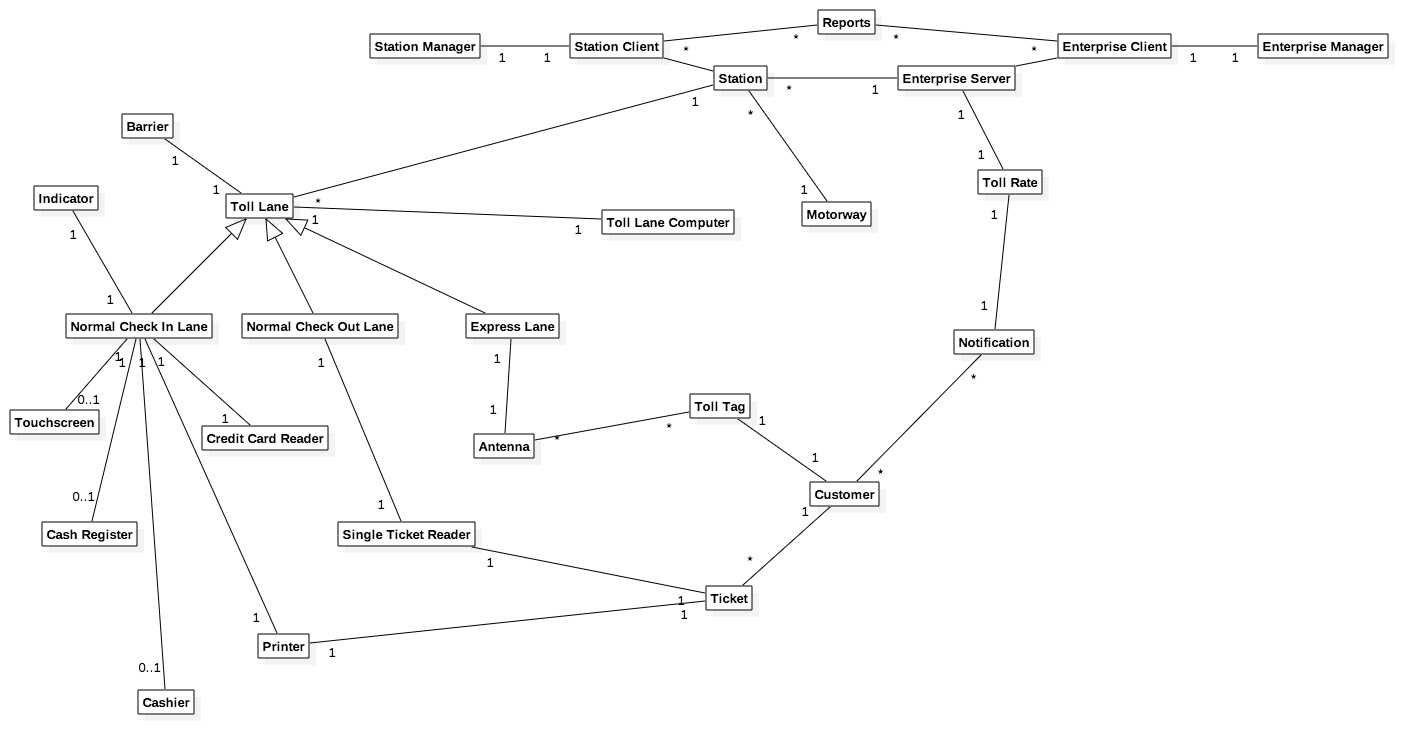
\includegraphics[width=1\textwidth]{figures/domain_model.jpg} 
  \end{center}
  \caption{Domain model diagram for the toll system}
\end{figure}
\section{Functional requirements}
The functional requirements have been identified for the system by looking at actions from the domain model and the game description.

\subsection{Use case diagram}
The use case diagram illustrates use cases in which actors interact with the system.

\begin{figure}[!ht]
  \begin{center}
    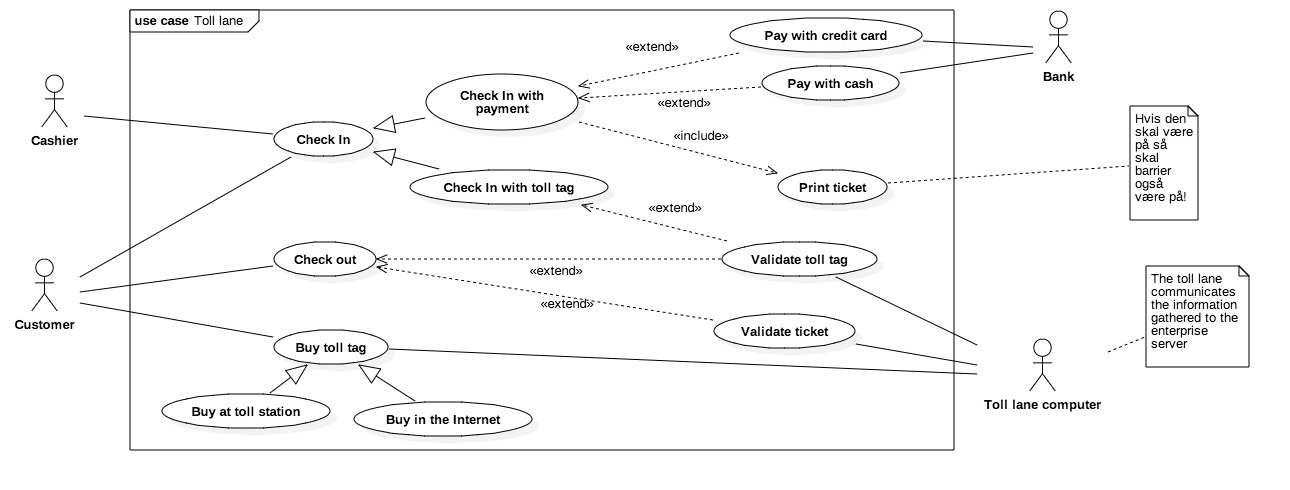
\includegraphics[width=1\textwidth]{figures/use_case_diagram.jpg} 
  \end{center}
  \caption{Use case diagram for the toll system}
\end{figure}

\subsection{Detailed use cases}
\subsubsection*{Check in with at cashier}

\begin{table}[H]
    \begin{tabular}{| p{3cm}| p{11.5cm}|}
        \hline
        
        Description             & The customer wants to check in on the toll motorway. \\\hline
        Actors                  & Customer, Cashier \\\hline
        Pre conditions          & The barrier is down. \\\hline
        
        Main Scenarios	        &
         
        \renewcommand{\labelenumi}{\arabic{enumi}.}
        \renewcommand{\labelenumii}{\Roman{enumii}:}
        
        \begin{enumerate}[topsep=0.0cm, leftmargin=0.5cm]
            \item The customer drives up to the cashier lane.
            \item The cashier chooses the sell ticket option in the system.
            \item The cashier chooses the vehicle type on the lane computer.
            \begin{enumerate}[partopsep=4cm, topsep=0cm, leftmargin=1cm]
                \item Wrong vehicle type.
        	\end{enumerate}
            \item The cashier chooses credit card or cash as payment type.
            \item The customer pays for the ticket.
            \begin{enumerate}[partopsep=4cm, topsep=0cm, leftmargin=1cm]
                \item The customers is not able to pay.
        	\end{enumerate}
        	\item The cashier prints the ticket.
        	\item The barrier opens.
        	\item The customer drives onto the toll road.
        	\item The barrier closes.
        \end{enumerate} \\\hline	
        
        Alternative Scenarios     & 
        
        \renewcommand{\labelenumi}{\Roman{enumi}:}
        \renewcommand{\labelenumii}{\alph{enumii})}
        
        \begin{enumerate}[a:, topsep=0.0cm,leftmargin=0.5cm]
            \item Wrong vehicle type.
        	\begin{itemize}[topsep=0cm, leftmargin=1cm]
        	    \item The cashier re-selects the vehicle type.
        	\end{itemize}
        	\item The customers is not able to pay.
        	\begin{itemize}[topsep=0cm, leftmargin=1cm]
        	    \item The customer gets a fine.
        	\end{itemize}
        \end{enumerate} \\\hline
        
        Post conditions         & The customer is checked-in on the toll road, with the correct vehicle type. Which is valid for 24 hours. \\\hline
        Notes                   & The ticket is only valid for one trip and only max 24 hours. The valid vehicle types is motorbike, car or truck. \\\hline
        
    \end{tabular}
    \caption{Detailed use case diagram - Check in with payment}
    \label{tab:UC1}
\end{table}
\subsubsection*{Check out with ticket}

\begin{table}[H]
    \begin{tabular}{| p{3cm}| p{11.5cm}|}
        \hline
        
        Description             & The customer wants to check out of the toll road with a ticket. \\\hline
        Actors                  & Customer, Cashier \\\hline
        Pre conditions          & Check in use case done, The barrier is down. \\\hline
        
        Main Scenarios	        &
         
        \renewcommand{\labelenumi}{\arabic{enumi}.}
        \renewcommand{\labelenumii}{\Roman{enumii}:}
        
        \begin{enumerate}[a:, topsep=0.0cm, leftmargin=0.5cm]
            \item The customer drives up to the normal check out lane.
            \item The customer inserts his ticket into the single ticket reader.
            \item The system validates the ticket.
            \begin{enumerate}[partopsep=4cm, topsep=0cm, leftmargin=1cm]
                \item Ticket has expired.
        	\end{enumerate}
        	\item The barrier opens.
        	\item The customer drives off the toll road.
        	\item The barrier closes.
        \end{enumerate} \\\hline	
        
        Alternative Scenarios     & 
        
        \renewcommand{\labelenumi}{\Roman{enumi}:}
        \renewcommand{\labelenumii}{\alph{enumii})}
        
        \begin{enumerate}[a:, topsep=0.0cm,leftmargin=0.5cm]
            \item Ticket has expired.
        	\begin{itemize}[topsep=0cm, leftmargin=1cm]
        	    \item The cashier performs correctly check out of the customer.
        	\end{itemize}
        \end{enumerate} \\\hline
        
        Post conditions         & The customer is checked out of the toll road. \\\hline
        Notes                   & The single ticket reader keeps the ticket after check out to avoid reuse of tickets. \\\hline
        
    \end{tabular}
    \caption{Detailed use case diagram - Check out with ticket}
    \label{tab:UC2}
\end{table}
\subsubsection*{Change rate on ticket price}

\begin{table}[H]
    \begin{tabular}{| p{3cm}| p{11.5cm}|}
        \hline
        
        Description             & The enterprise manager wants to change rate for the ticket price, using the enterprise client.  \\\hline
        Actors                  & Enterprise manager \\\hline
        Pre conditions          & The enterprise manager is logged in. \\\hline
        
        Main Scenarios	        &
         
        \renewcommand{\labelenumi}{\arabic{enumi}.}
        \renewcommand{\labelenumii}{\Roman{enumii}:}
        
        \begin{enumerate}[a:, topsep=0.0cm, leftmargin=0.5cm]
            \item The enterprise manager navigates to the change rate section.
            \item The enterprise manager selects to change the ticket price.
            \item The enterprise manager edits the ticket price.
            \begin{enumerate}[partopsep=4cm, topsep=0cm, leftmargin=1cm]
                \item Invalid price for ticket.
        	\end{enumerate}
        	\item The price gets changed for all stations.
        \end{enumerate} \\\hline	
        
        Alternative Scenarios     & 
        
        \renewcommand{\labelenumi}{\Roman{enumi}:}
        \renewcommand{\labelenumii}{\alph{enumii})}
        
        \begin{enumerate}[a:, topsep=0.0cm,leftmargin=0.5cm]
            \item Invalid price for ticket.
        	\begin{itemize}[topsep=0cm, leftmargin=1cm]
        	    \item The system indicates that the prices is invalid.
        	\end{itemize}
        \end{enumerate} \\\hline
        
        Post conditions         & The price is changed for all stations. \\\hline
        Notes                   & The ticket price can't be under zero. \\\hline
        
    \end{tabular}
    \caption{Detailed use case diagram - Change rate}
    \label{tab:UC3}
\end{table}
\subsubsection*{Show report}

\begin{table}[H]
    \begin{tabular}{| p{3cm}| p{11.5cm}|}
        \hline
        
        Description             & The station manager wants to see statistical reports from the station client. \\\hline
        Actors                  & Station Manager \\\hline
        Pre conditions          & Sign in use case done. \\\hline
        
        Main Scenarios	        &
         
        \renewcommand{\labelenumi}{\arabic{enumi}.}
        \renewcommand{\labelenumii}{\Roman{enumii}:}
        
        \begin{enumerate}[a:, topsep=0.0cm, leftmargin=0.5cm]
            \item The station manager navigates to the report section in the client.
            \item The station manager fills out the query conditions for the report.
            \item The station manager requests a report.
            \begin{enumerate}[partopsep=4cm, topsep=0cm, leftmargin=1cm]
                \item Not all the required information is filled out.
        	\end{enumerate}
        	\item A report of the given period is displayed.
        \end{enumerate} \\\hline	
        
        Alternative Scenarios     & 
        
        \renewcommand{\labelenumi}{\Roman{enumi}:}
        \renewcommand{\labelenumii}{\alph{enumii})}
        
        \begin{enumerate}[a:, topsep=0.0cm,leftmargin=0.5cm]
            \item Not all the required information is filled out.
        	\begin{itemize}[topsep=0cm, leftmargin=1cm]
        	    \item The station client displays an error message.
        	\end{itemize}
        \end{enumerate} \\\hline
        
        Post conditions         & The station client displays the requested report. \\\hline
        Notes                   & The statistics will include how many single tickets were used and how often toll tags were used, for each type of vehicle. \\\hline
        
    \end{tabular}
    \caption{Detailed use case diagram - Show report}
    \label{tab:UC4}
\end{table}

\section{Non Functional requirements}
Non functional requirements have been identified for the toll system and will be discussed further in this section.

\begin{table}[H]
    \begin{tabular}{| l | p{12cm} | l |}
        \hline
        \#  & \textbf{Requirements} & \textbf{\underline{Approved}} \\\hline
        1.  & The barrier may only let \textbf{\underline{one}} car through at a time & \\\hline
        2.  & The barrier must \textbf{\underline{not}} close before a car has passed through & \\\hline
        3.  & The barrier must be able to \textbf{\underline{withstand}} a moving car & \\\hline
        4.  & The system runs on a \textbf{\underline{Linux}} distribution & \\\hline
        5.  & Toll tag users should be able to drive through the station with \textbf{\underline{30 km/h}} & \\\hline
        6.  & Buying tickets at the station should be \textbf{\underline{anonymous}} & \\\hline
        7.  & The interface on the toll lane computer should be \textbf{\underline{intuitive}} for the cashier & \\\hline
        8.  & In case of malfunction barrier, the personal should be able to \textbf{\underline{manually}} open and close the barrier & \\\hline
    \end{tabular}
    \caption{Non functional requirements for the toll system}
    \label{tab:non-functional}
\end{table}



\chapter{Acceptance test}
In this section the group have created acceptance tests for the four selected use cases of the toll system. The acceptance test is written as fit-tests.

\subsection{Acceptance test - Check in at cashier}
The pick up object tests, test if the player is able to pick up objects in the game.

\begin{table}[H]
    \centering
    \begin{tabular}{| l | l | l |}
        \hline
        \textbf{ActionFixture} &  &  \\\hline
        Start & TollSystem &  \\\hline
        Check & barrier is down & true  \\\hline
        Check & customer in lane & true  \\\hline
        Press & sell ticket &  \\\hline
        Enter & vehicle type & car \\\hline
        Enter & payment method & cash \\\hline
        Enter & & \\\hline
    \end{tabular}
    \caption{Fit test for Check in at cashier}
\end{table}
\subsection{Acceptance test - Check out with ticket}
Check out with a single ticket.

\begin{table}[H]
    \centering
    \begin{tabular}{| l | l | l |}
        \hline
        \textbf{ActionFixture}  &                       & \\\hline
        Check                   & The barrier is down   & true  \\\hline
        Check                   & Ticket is valid       & true  \\\hline
        Check                   & The barrier opens     & true  \\\hline
        Check                   & Car goes through      & true \\\hline
        Check                   & The barrier closes    & true \\\hline
       
    \end{tabular}
    \caption{Fit test for Pick up object}
\end{table}

First alternative scenario. The ticket is not valid.

\begin{table}[H]
    \centering
    \begin{tabular}{| l | l | l |}
        \hline
        \textbf{ActionFixture}  &                           & \\\hline
        Check                   & The barrier is down       & true  \\\hline
        Check                   & Ticket is valid           & false  \\\hline
        Enter                   & Reason for invalidation   & Slept at highway hotel  \\\hline
        Press                   & Open gate button          & \\\hline
        Check                   & The barrier opens         & true  \\\hline
        Check                   & Car goes through          & true \\\hline
        Check                   & The barrier closes        & true \\\hline
       
    \end{tabular}
    \caption{Fit test for Pick up object}
\end{table}
\subsection{Acceptance test - Change Rate}
Change rate tests, test if the enterprise manager is able to rate for the ticket price.

\begin{table}[H]
    \centering
    \begin{tabular}{| l | l | l |}
        \hline
        \textbf{Action Fixture} &                                                               &       \\\hline
        Start                   & Enterprise manager is logged in                               & true  \\\hline
        Enter                   & Enterprise manager navigates to the change rate section       &       \\\hline
        Check                   & New ticket price                                              & 80    \\\hline
        Press                   & Enterprise manager selects to change the ticket price         &       \\\hline
        Enter                   & Enterprise manager inputs new ticket price                    & 100   \\\hline
        Press                   & Enterprise manager updates ticket price                       & true  \\\hline
        Check                   & New ticket price                                              & 100   \\\hline
    \end{tabular}
    \caption{Fit test for Change Rate}
\end{table}

\subsubsection{Alternative Scenario - Invalid price for ticket}
\begin{table}[H]
    \centering
    \begin{tabular}{| l | l | l |}
        \hline
        \textbf{Action Fixture} &                                                               &       \\\hline
        Start                   & Enterprise manager is logged in                               & true  \\\hline
        Enter                   & Enterprise manager navigates to the change rate section       &       \\\hline
        Check                   & New ticket price                                              & 80    \\\hline
        Enter                   & Enterprise manager selects to change the ticket price         &       \\\hline
        Press                   & Enterprise manager inputs new ticket price                    & -100  \\\hline
        Press                   & Enterprise manager updates ticket price                       & false \\\hline
        Check                   & Error message                                                 & Invalid ticket price \\\hline
    \end{tabular}
    \caption{Fit test for Change Rate}
\end{table}
\subsection{Acceptance test - Show report}

\textbf{Usecase "Show report"success scenario.}

\begin{table}[H]
    \centering
    \begin{tabular}{| l | l | l |}
        \hline
        \textbf{ActionFixture}   & & \\\hline
        start                    & station client & \\\hline
        enter                    & start date     & 06/01/17\\\hline
        enter                    & end date       & 06/08/17\\\hline
        press                    & request report & \\\hline
        check                    & error message  & none \\\hline
    \end{tabular}
    \caption{Success scenario}
\end{table}

\textbf{First alternative scenario: Not all the information is filled out}

\begin{table}[H]
    \centering
    \begin{tabular}{| l | l | l |}
        \hline
        \textbf{ActionFixture}   & & \\\hline
        start                    & station client & \\\hline
        enter                    & start date     & 06/01/17\\\hline
        enter                    & end date       & \\\hline
        press                    & request report & \\\hline
        check                    & error message  & no end date has been entered \\\hline
    \end{tabular}
    \caption{Alternative scenario}
\end{table}




\chapter{Design}
\section{Non-Trivial Design Decisions}

This subsection describes non-trivial design decisions and any assumptions made for the design of the system. The subsection is divided into three different sections for each major design decision, using the following format:

\begin{itemize}
    \item The challenge in the design
    \item Alternatives to the chosen design
    \item Why the selected solution
\end{itemize}

\subsubsection*{Challenge in the design}
When designing an online multiplayer game some challenges with keeping the game world in sync on all the clients arises. The game servers responsibility is to keep this shared game world state, due to this design each client (phone) has to request the game world state which can be very computational hard if the game world is very big. 

\subsubsection*{Alternatives}
One solution to the shared game world state could be to create a game controller class on the client (phone) which stores all information about the game world and which syncs with the game server, when changes happens. This doesn't solve the computational problem though.

\subsubsection*{The selected solution}
To keep the design simple and to overcome computational problems, each client (phone) only stores a single room in memory at a time.
\section{Component design}
In this section a high level component design is represented and shown in figure \ref{fig:high-level-component}. The component diagram shows the communication between the two components in the system, a phone and the game server.


\subsection*{High level component view}
The game server provides a interface for the phone to use and there by logon to the game. Futhere more the interface provides functionality for trading items and picking up items in the game. 

\begin{figure}[!ht]
  \begin{center}
    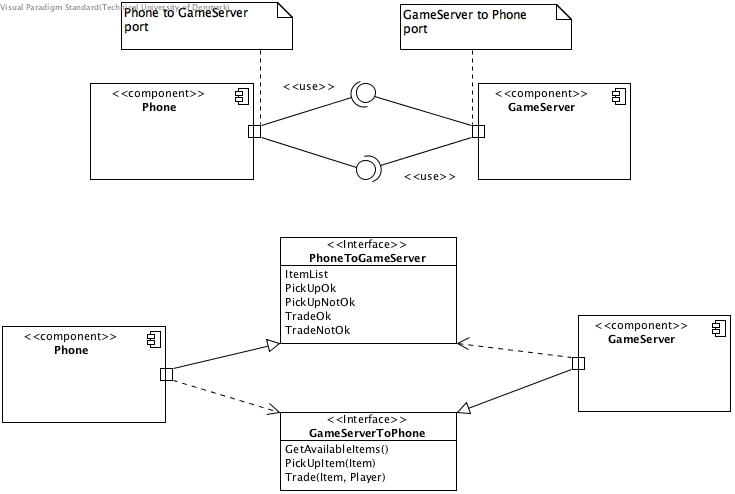
\includegraphics[width=1\textwidth]{figures/high-level-view.jpg} 
  \end{center}
  \caption{High level component view of the MUD Game}
  \label{fig:high-level-component}
\end{figure}

\section{Detailed class design}
In this subsection of the design a detailed class diagram for the two use cases figure \ref{tab:UC1}. and figure \ref{tab:UC2}. is presented. Here it shows that the player is only aware of the game state in which room he is in, the rest is unknown.

\begin{figure}[!ht]
  \begin{center}
    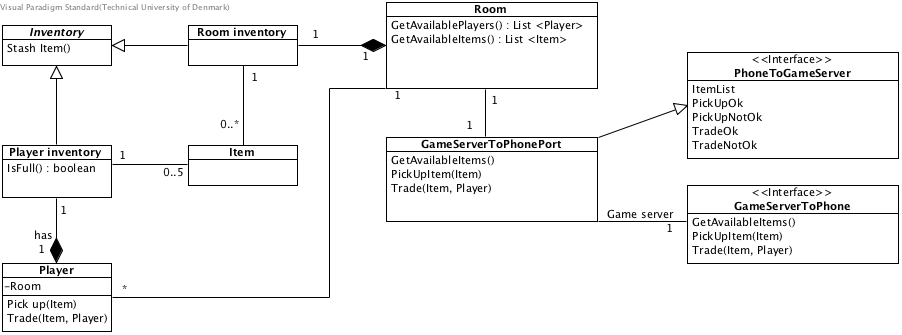
\includegraphics[width=1\textwidth]{figures/class_diagram.jpg} 
  \end{center}
  \caption{Detailed class diagram of the MUD Game}
  \label{fig:class-diagram}
\end{figure}

\section{Behaviour design}
Describe the behaviour of each class using state machines.

\chapter{Validation}

\section{Use Case Realisation}

\chapter{conclusion}
Our experience with the project goes here...

\section{Notes delete me before hand-in}

\textbf{Actors of the system}
\begin{itemize}
    \item The cashier
    \item The station manager
    \item The enterprise manager
    \item The customer
\end{itemize}

\textbf{Use cases selected for dev.}
\begin{itemize}
    \item Check-in
    \item Check-out
    \item Change rate
    \item Show reports
\end{itemize}

\end{document}
